\chapter{Efficient knockoffs construction}\label{ch:sdp}

As shown in Chapter~\ref{ch:knockoffs}, in the case of gaussian knockoffs,
$\tX$ can be sampled from a normal distribution $\cN\left( \bupsilon,\, \Upsilon \right)$ whose parameters
$\bupsilon,\, \Upsilon$ are formulated in~\ref{eq:conditional_gaussian_knockoffs2}.
\begin{equation}\label{eq:conditional_gaussian_knockoffs2}
    \tcX \mid \cX \sim \cN\left( \bupsilon, \Upsilon \right)
    ,\qquad\text{where}\quad
    \begin{cases*}
        \bupsilon = \cX - \cX\Sigma^{-1}\diag\{ \bs \}\\
        \Upsilon = \diag\{ \bs \}\left( 2I_{p \times p} - \Sigma^{-1}\diag\{ \bs \} \right)
    \end{cases*}
\end{equation}
More generally, the same parameters are derived by only imposing
$\big[ X, \tX \big]_{\swap\left( S \right)}$ and $\big[ X, \tX \big]$
to have equal first two moments
for any subset
$S \subseteq \left\{ 1, \dots, p \right\}$,
rather than the same distribution.
These formulas are valid for any vector $\bs \in \R^p$ such that $\Omega$
is indeed a covariance matrix (semidefinite positive).
\begin{equation*}
    \Omega = \begin{bmatrix}
        \Sigma & \Sigma - \diag \bs\\
        \Sigma - \diag \bs & \Sigma
    \end{bmatrix}
    \succeq \0_{2p \times 2p}
\end{equation*}
As shown in Proposition~\ref{prop:omega_psd},
this matrix is semidefinite positive if and only if $\0_{p \times p} \preceq \diag \bs \preceq 2 \Sigma$.
The first inequality clearly holds if all the entries of $\bs$ are positive.
It is however trickier to identify all vectors $\bs$ satisfying the second one.

In this chapter, we show why the choice of $\bs$ is important and how to efficiently find an appropriate one
in the high-dimensional setting.
We also form low-rank covariance approximations and procedures to quickly sample $\tcX$.
In the remaining, we note $\Sigma$ the true covariance and $\hat{\Sigma}$ its estimation from the samples $X$
(be it empirical or derived from more sophisticated methods).

\section{Equi-correlated knockoffs}\label{sec:equi}

\subsubsection{A cheap solution}

For any psd matrix $A \in \R^p$, $A + \alpha I_{p \times p}$ has the same eigenvalues as $A$, but shifted by $\alpha$.
It gives a fast and simple way to find a feasible $\bs$:
setting all the entries to the smallest eigenvalue of $\tcove$ (\textit{equi}-correlated knockoffs).
\begin{equation}\label{eq:equi}
    s_j = 2\lambda_{\min}(\cove)
    \quad\text{for all}\quad 0 \leq j \leq p
\end{equation}
The problem of finding the smallest eigenvalue $\lambda_{\min}(\cove)$ can be solved efficiently,
using for instance a singular value decomposition which runs in $\cO(p^3)$ steps~\citep{svd}.

\subsubsection{Why it is not desirable}

For large values of $p$,
the minimum eigenvalue of $\cove$ is likely to be very small,
unless $\cove$ has a substantially special structure.
Let us analyze briefly the covariance of $\big[ \cX; \tcX \big]$
to understand why it is unprofitable for the selection procedure.
If $\tcX$ is built according to~\ref{eq:conditional_gaussian_knockoffs2}, it satisfies
\begin{equation*}
    \begin{cases}
        \cov(\tcX_j,\, \tcX_{j'}) = \cov(\cX_j,\, \cX_{j'}) \text{ for all } j,\,j'\\
        \cov(\cX_j,\, \tcX_{j'}) = \cov(\cX_j,\, \cX_{j'}) \text{ for all } j \neq j'\\
        \cov(\cX_j,\, \tcX_j) = \cov(\cX_j,\, \cX_j) - s_j \text{ for all } j
    \end{cases}
\end{equation*}
First, $\tcX$ has the same internal covariance has $\cX$,
and two distinct original and knockoff features have the same covariance
as the one of the two corresponding original features.
It makes the knockoff features sufficiently close to the original features
to fool the estimator computing the statistics.
However, an original feature $j$ and its corresponding knockoff have a covariance that is smaller the larger $s_j$ is.
If $s_j$ is close to $0$,
$\cX_j$ cannot be distinguished from $\tcX_j$ and the selection is prone to suffer from a low power.
This fact is even more detrimental when $p$ is large as $\lambda_{\min}$ is likely to be very close to $0$.

\section{SDP knockoffs}\label{sec:sdp}

The observation of the previous Section~\ref{sec:equi} motivates us to maximize the entries of $\bs$,
while maintaining the inequality $\diag\bs \preceq \tcovm$.
This can be formulated in the optimization problem~\ref{eq:sdp}.
\begin{equation}\label{eq:sdp}
    \underset{\bs \in \R^p}{\argmax}\;\,
    \sum_{j = 1}^p s_j
    \qquad
    \text{subject to}\quad \begin{cases}
        s_j \geq 0\text{ for all } j\\
        \diag \bs \preceq \tcove
    \end{cases}
\end{equation}
This problem is a structured semidefinite program (SDP) and can be solved efficiently for small values of
$p$ by interior point methods~\citep{sdo_todd, sdp_handbook} for example.
However, it quickly becomes intractable for large values of $p$ (one thousand or more).
In memory, these schemes need to store roughly $\cO(m^2)$ floats
and the time complexity is approximately $\cO\left( m^3 \right)$, where $m$ is the number of constraints
($p$ is this case).
Experimentally, alternating direction~\citep{sdp_admm}
and first order methods like SCS~\citep{sdp_scs} also fail to scale satisfactorily in high dimension.
Figure~\ref{fig:cvx_sdp_times} shows the convergence time of the solvers SCS and MOSEK as a function of $p$.
It makes it clear that different approaches have to be considered when $p$ is more than a few thousands.
Moreover, most solutions returned by these algorithms are actually infeasible because of numerical approximations.
\begin{figure}
    \centering
    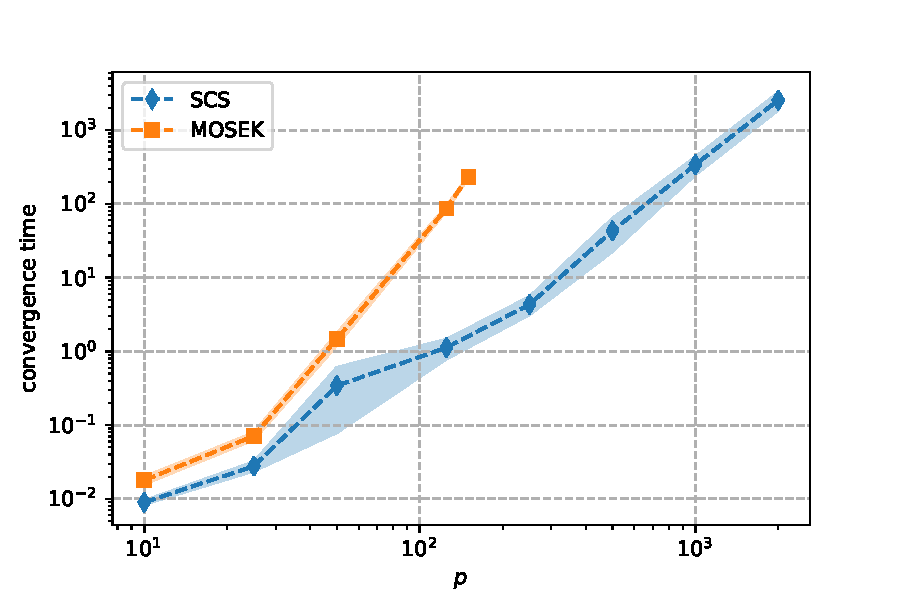
\includegraphics[width=0.8\linewidth, height=0.5\linewidth]{figures/cvx_sdp_times.pdf}
    \caption{
        Time (in seconds) required to converge for SCS (blue) and MOSEK (orange) solvers
        as a function of $p$ in log-log scale.
        Rapidly, MOSEK needs too much memory and can't be run for $p > 150$.
        Both match the theoretical $\cO(p^3)$ rate and SCS already needs 15 minutes for $p = 1000$.
        See Appendix~\ref{sec:cvx_times} for details regarding the random generation of covariance
        matrices $\cove$.
    }
    \label{fig:cvx_sdp_times}
\end{figure}

In order to reduce the computation time~\cite{model_x_knockoffs}
suggest to solve an approximated problem of~\ref{eq:sdp} in 2 steps that we describe below.
\paragraph*{Step 1.}
Pick a block-diagonal approximation $\coveapprox$ of $\cove$ and solve
\begin{equation}\label{eq:sdp_approx}
    \underset{\hat{\bs} \in \R^p}{\argmax}\;\,
    \sum_{j = 1}^p \hat{s}_j
    \qquad
    \text{subject to}\quad \begin{cases}
        \hat{s}_j \geq 0\text{ for all } j\\
        \diag \hat{\bs} \preceq \tcoveapprox
    \end{cases}
\end{equation}
\paragraph*{Step 2.}
Solve the one dimensional maximization
\begin{equation}\label{eq:sdp_approx_1d}
    \underset{\gamma \in \R}{\argmax}\;\,\gamma
    \qquad\text{subject to}\quad
    \diag\left( \gamma \cdot \hat{\bs} \right) \preceq \tcove
\end{equation}
Finally, pick $\bs = \gamma \cdot \hat{\bs}$.
\begin{remark}
    Note that the two extreme options $\coveapprox = I$ and $\coveapprox = \cove$ yield
    the same solutions as solving equi-correlated knockoffs~\ref{eq:equi} and full SDP knockoffs~\ref{eq:sdp} respectively.
\end{remark}
Solving~\ref{eq:sdp_approx_1d} in Step 2 can be done very efficiently using bisection as it is a one-dimensional SDP\@.
The optimization problem~\ref{eq:sdp_approx} is the same as the one in~\ref{eq:sdp},
except for the approximation $\coveapprox$.
To speed up the computations,
$\coveapprox$ can be chosen to be a block-diagonal matrix of $k$ blocks.
The maximization then reduces to $k$ smaller SDPs for which solutions can be found more efficiently.
All the sub-problems being independent, they could even be distributed in several computation nodes.
Picking $\coveapprox$ is a compromise between available computation time and quality of the approximation
(hence ultimate statistical power of the procedure).
The block-diagonal structure can be obtained by reordering columns of $\cove$
with a clustering step grouping similar features (i.e. highly correlated features).

\bigbreak
In practice, the block-diagonal structure is unrealistic.
On top of that, the problem remains intractable when $p$ is a few dozens of thousands,
even if ten groups of features are identified.
The clustering step may also be costly,
and the covariance matrix $\cove$ itself might not even be storable in memory.

\section{A coordinate ascent approach}\label{sec:coordinate_ascent}

We propose here a coordinate ascent algorithm which is proven to converge when coupled with a log-barrier penalty.
It may very well be executed in the block-diagonal arrangement depicted in the previous section.

\subsection{Notations and preliminaries}\label{subsec:notations_preliminaries}

\paragraph{Notations.}
Let $M \in \R^{p \times p}$.
Given two sets of indices $\cI,\,\cJ \in \fset$,
we note $M_{\cI,\,\cJ}$ the $\abs{\cI} \times \abs{\cJ}$ matrix obtained by keeping
the $\abs{\cI}$ rows and $\abs{\cJ}$ columns indexed by $\cI$ and $\cJ$ respectively.
By convenience, an integer $j$ denotes the set $\left\{ j \right\}$ and $j^c$ $\fset \setminus \left\{ j \right\}$
in the matrix subscripting context.
For example, if $M = \begin{bmatrix}
    1 & 2 & 3\\
    4 & 5 & 6\\
    7 & 8 & 9
\end{bmatrix}$,
then $M_{1^c, 1^c} = \begin{bmatrix}
    5 & 6\\
    8 & 9
\end{bmatrix}$
and $M_{1^c, 1} = \begin{bmatrix}
    4\\
    7
\end{bmatrix}$.

\paragraph{Positiveness characterisation.}
Suppose $M$ is structured as
\begin{equation*}
    M = \begin{bmatrix}
        \xi & \yy^\top\\
        \yy & B
    \end{bmatrix}
\end{equation*}
where $B$ is symmetric and invertible.
\begin{lemma}\label{lemma:schur1}
    Using Schur complements (see Appendix~\ref{sec:schur_complement}), it holds that M is psd if and only if
    \begin{equation*}
        B \succeq \0
        \quad\text{and}\quad
        \xi - \yy^\top B^{-1} \yy \geq 0
    \end{equation*}
\end{lemma}
In subscript notations, this is equivalent to $M_{1^c,\, 1^c} \succeq \0$ and
$M_{1,\, 1} - M_{1^c,\, 1}^\top M_{1^c,\, 1^c} M_{1^c,\, 1} \geq 0$.
This statement can be generalized as follows.
For any $j \in \fset$, M is psd if and only if both conditions in~\ref{eq:psd_schur_permutation} are satisfied
\begin{equation}\label{eq:psd_schur_permutation}
    \begin{cases}
        M_{j^c,\, j^c} \succeq \0\\
        M_{j,\, j} - M_{j^c,\, j}^\top M_{j^c,\, j^c} M_{j^c,\, j} \geq 0
    \end{cases}
\end{equation}
\begin{proof}
    Let $j \in \fset$.
    Let $P$ be the permutation matrix swapping columns $1 \leftrightarrow j$ and letting other columns unchanged.
    In two-line form, it is written
    \begin{equation*}
        P = \begin{pmatrix}
                1 & 2 & \dots & j - 1 & j & j + 1 & \dots & p\\
                j & 2 & \dots & j - 1 & 1 & j + 1 & \dots & p
        \end{pmatrix}
    \end{equation*}
    M is psd if and only if $P^\top M P$ is psd.
    $P^\top M P$ is $M$ with lines and columns $1$ and $j$ swapped.
    By applying Lemma~\ref{lemma:schur1} on it, we get the result.
\end{proof}

\subsection{Coordinate ascent}\label{subsec:coordinate_ascent}

Using the characterization~\ref{eq:psd_schur_permutation},
it appears that the feasibility of $\bs$ in SDP~\ref{eq:sdp} is equivalent to the three following conditions,
for any $j \in \fset$
\begin{equation}\label{eq:schur_sdp_constraints}
    \tcove \succeq \diag \bs \succeq \0
    \iff
    \begin{cases}
        \bs \geq \0\\
        \tcove_{j,\, j} - s_j
            - 4\cove_{j^c,\, j}^\top\big( \tcove_{j^c,\, j^c} - \diag \bs_{j^c} \big)^{-1}\cove_{j^c,\, j} \geq 0\\
        \tcove_{j^c,\, j^c} - \diag \bs_{j^c} \succeq \0
    \end{cases}
\end{equation}
This observation motivates the following coordinate approach, as described by~\cite{block_coordinate_sdp}.
Start with a feasible solution $\bs_0$, for example $\bs_0 = \0_p$.
At each iteration, only one coordinate $j$ of $\bs$ will be updated (to optimize a sub-objective),
and the constraints remain satisfied if we pick $s_j$ such that
\begin{equation}\label{eq:sdp_simple_constraints}
    \begin{cases}
        s_j \geq 0\\
        s_j \leq \tcove_{j,\, j}
            - 4\cove_{j^c,\, j}^\top\big( \tcove_{j^c,\, j^c} - \diag \bs_{j^c} \big)^{-1}\cove_{j^c,\, j}
    \end{cases}
\end{equation}
Consequently, we set $s_j$ to the maximum value keeping the constraints valid,
that is
\begin{equation*}
s_j = \max\Big( \tcove_{j,\, j}
    - 4\cove_{j^c,\, j}^\top\big( \tcove_{j^c,\, j^c} - \diag \bs_{j^c} \big)^{-1}\cove_{j^c,\, j}
    ,\, 0 \Big)
\end{equation*}
Unfortunately, this method is not guaranteed to converge to the global maximum, even when the problem is concave.
A slight modification depicted in the next section will correct that.

\subsection{Log-barrier}\label{subsec:log_barrier}

Instead of optimizing~\ref{eq:sdp},
we absorb the constraint $\tcove \succeq \bs$ into the objective by penalizing solutions
too close to the feasibility frontier, as described by~\citet[§11.3]{convex_optimization}.
It depends on the additional term
$\lambda \cdot \log\det\big( \tcove - \diag\bs \big)$
for some coefficient $\lambda > 0$:
\begin{equation}\label{eq:sdp_log_barrier}
    \underset{\bs \in \R^p}{\argmax}\;\,
    \sum_{j = 1}^p s_j
    + \lambda \cdot \log\det\big( \tcove - \diag\bs \big)
    \qquad
    \text{subject to}\quad
    s_j \geq 0\text{ for all } j
\end{equation}
where we consider that $\log 0 = -\infty$.
Intuitively, a solution $\bs$ such that the minimum eigenvalue of $\tcove - \diag\bs$ gets too close to $0$
will be penalized by this $\log$ term.

\bigbreak
The following lemma will be helpful to compute the determinant.
\begin{lemma}
    If $M = \begin{bmatrix}
        \xi & \yy^\top\\
        \yy & B
    \end{bmatrix}$,
    then
    \begin{align*}
        \det\left( M \right) &= \det\big( \xi - \yy^\top B^{-1} \yy \big) \cdot \det\left( B \right)\\
        &= \big( \xi - \yy^\top B^{-1} \yy \big) \cdot \det\left( B \right)
    \end{align*}
\end{lemma}
\begin{proof}
    It is an immediate consequence of the formula giving the determinant of a block matrix
    reported in Appendix~\ref{sec:block_matrix_det}.
\end{proof}
With subscript notations, this identity can be noted as
$\det\left( M \right) = \big( M_{1,\, 1} - M_{1^c,\, 1}^\top M_{1^c,\, 1^c}^{-1} M_{1^c,\, 1} \big)
    \cdot\det\left( M_{1^c,\, 1^c} \right)$.
Employing the same idea as in~\ref{eq:psd_schur_permutation},
it can further be generalized to
\begin{equation*}
    \det\left( M \right) = \big( M_{j,\, j} - M_{j^c,\, j}^\top M_{j^c,\, j^c}^{-1} M_{j^c,\, j} \big)
        \cdot\det\left( M_{j^c,\, j^c} \right)
\end{equation*}
for any $j \in \fset$.
By applying this to $\log\det\big( \tcove - \diag\bs \big)$,
we get that for any $j$,
\begin{equation*}
    \log\det\big( \tcove - \diag\bs \big) =
        \log\big( \tcove_{j,\, j} - s_j - 4\cove_{j^c,\, j}^\top Q_j^{-1} \cove_{j^c,\, j} \big)
            + \log\det\left( Q_j \right)
\end{equation*}
where $Q_j = \tcove_{j^c,\, j^c} - \diag\bs_{j^c}$ does not depend on $s_j$.

\bigbreak
Again, we start from a feasible solution $\bs^{(0)} = \0_p$ and perform coordinate ascent.
At each iteration, a new coordinate $j$ is updated
and we take advantage of the fact that $Q_j$ doesn't depend on $s_j$.
The function
\begin{equation*}
    \alpha \mapsto \alpha
        + \lambda\log\big( \tcove_{j,\, j} - \alpha - 4\cove_{j^c,\, j}^\top Q_j^{-1} \cove_{j^c,\, j} \big)
\end{equation*}
is concave and setting its derivative to $0$ yields that its maximum is
\begin{equation*}
    \alpha^\star = \tcove_{j,\, j} - 4\cove_{j^c,\, j}^\top Q_j^{-1} \cove_{j^c,\, j} - \lambda
\end{equation*}
The $j$th coordinate is therefore updated as $s_j \leftarrow \max\left( \alpha^\star,\, 0 \right)$.
Note in particular that this update maintains the feasibility
conditions~\ref{eq:sdp_simple_constraints} for any value of $\lambda$.

\citet[§11.3]{convex_optimization} suggest that picking $\lambda = \epsilon / p$ will yield an
$\epsilon$-optimal solution.
In practice, an initial $\lambda_0$ is picked and it is multiplied by a decay rate
$0 < \mu < 1$ after each coordinate cycle to refine the solution.
This scheme can be proven to converge to the maximum
of the modified objective~\ref{eq:sdp_log_barrier}.
It is indeed a particular case of ~\citet[Theorem~3]{block_coordinate_sdp},
which applies in this case as the constraints are simple,
i.e. $\bs \geq \0$ is of the form $L \leq \diag\bs \leq U$.

\bigbreak
This log-barrier algorithm is summarized in pseudo-code in Algorithm~\ref{alg:coordinate_ascent_log_barrier}.
The bottleneck is the inversion of the matrix
$Q_j \in \R^{(p - 1) \times (p - 1)}$ in line~\ref{alg:line:q_inv} which takes $\cO\left( p^3 \right)$ steps.
As it is done in every inner iteration, the time complexity of Algorithm~\ref{alg:coordinate_ascent_log_barrier} is
$\cO\left( n_\text{iters} \cdot p^4 \right)$ when implemented naively.
It is possible to design a version running in $\cO\left( n_\text{iters} \cdot p^3 \right)$ steps instead.
To see this, note $A = \tcove - \diag\bs \in \R^{p \times p}$.
At each iteration $j$, $Q_j$ is a principal sub-matrix of $A$ and its inverse can efficiently be computed
(in $\cO\left( p^2 \right)$ steps) from the one of $A$~\citep{submatrix_inverse}.
On top of that, when a coordinate $s_j$ changes,
$A$ is only modified with a rank-$1$ update.
Its new inverse can efficiently be computed ($\cO\left( p^2 \right)$ steps)
using for example Sherman-Morrison formula
(see Appendix~\ref{ch:linear_algebra})
or Cholesky rank-$1$ updates~\citep{cholesky_rank_1} which are more stable numerically.
In Appendix~\ref{ch:cython_acceleration} we give a Cython implementation example.
\begin{algorithm}[t]
    \caption{Coordinate ascent with log-barrier}\label{alg:coordinate_ascent_log_barrier}
    \begin{algorithmic}[1]
        \State \textbf{Input:} $\cove$, barrier coefficient $\lambda$, decay $\mu$, $\bs^{(0)} = \0_p$
        \State $\bs = \bs^{(0)}$
        \Repeat
        \For{$j = 1,\,\dots,\, p$}
        \State $Q_j = \tcove_{j^c,\, j^c} - \diag\bs_{j^c}$
        \State $s_j = \max\big( \tcove_{j,\, j} - 4\cove_{j^c,\, j}^\top Q_j^{-1} \cove_{j^c,\, j} - \lambda,\, 0 \big)$\label{alg:line:q_inv}
        \EndFor
        \State $\lambda = \mu \cdot \lambda$
        \Until{stopping criteria}
    \end{algorithmic}
\end{algorithm}

\section{Low-rank covariance approximation}\label{sec:low_rank_sigma}

Covariance estimation in the high-dimensional setting ($p > n$ where $n$ is the number of samples)
is challenging as the sample (empirical) covariance is not accurate.
On top of that,
if $p$ is larger than $20\,000$ it becomes challenging to solely store the full matrix in the memory
of a standard computer.
Hopefully, big data matrices and especially correlation matrices often have an underlying low-rank structure,
or at least can be approximated adequately by such a low-rank estimate~\citep{big_data_low_rank}.
An intuitive explanation is that only a small number of latent features explain most of the data.

\subsection{Factor model}\label{subsec:factor_model}

We approximate the covariance $\cove$ with the following structure
\begin{equation}\label{eq:low_rank_structure}
    \cove = D + U \Lambda U^\top
\end{equation}
where $U \in \R^{p \times k}$ has orthogonal columns ($U^\top U = I_k$),
and both $D \in \R^{p \times p},\, \Lambda \in \R^{k \times k}$
are diagonal and psd.
$k$ is typically much lower than $p$ to save has much memory and computations as possible.

In the case where $X$ is reasonably large,
the decomposition~\ref{eq:low_rank_structure} for the empirical covariance can be obtained as follows.
First factorize $X = P \Delta Q^T$ with SVD~\citep{svd}.
Then (assuming columns are centered),
\begin{align*}
    \cove &= \frac{1}{n}X^\top X\\
    &= \frac{1}{n}Q \Delta^2 Q^\top
\end{align*}
From this, building a rank-$k$ approximation of $\cove$ is easily done by keeping its top $k$ eigenvalues,
that is
\begin{equation*}
    \Lambda = \Delta^2_{:k,\, :k} \qquad\qquad U = Q_{:,\, :k}
\end{equation*}
Then set $D = \diag^2\max \big( \cove - U \Lambda U^\top,\, \0_{p \times p} \big)$
to be the diagonal psd matrix containing
the difference between $\cove$ and the low-rank approximation.
None of these steps requires to form the full covariance matrix $\cove$, which might not fit in memory.

As pointed out earlier, the empirical covariance estimator performs poorly in high dimension.
Shrunk estimators like the one proposed by~\cite{ledoit_wolf} are proven to be often superior in that situation.
Suppose again that $\cove = \frac{1}{n}X^\top X$ is the empirical estimator.
Note $\mu = \Tr( \cove ) / p$ and $\delta$ a shrinkage coefficient.
The shrunk covariance estimator is then given by
\begin{equation*}
    \cove_\delta = (1 - \delta)\cove + \delta\mu I
\end{equation*}
The same decomposition strategy can be employed,
but this time $\cove_\delta = Q\big[ (1 - \delta) \Delta^2 / n + \delta\mu I \big] Q^\top$.
Finding the optimal coefficient $\delta$ can be done in $\cO\left( n \cdot p \right)$ steps
and without extra memory, provided that we know the decomposition of $X$.

Randomized SVD algorithms~\citep{random_svd} may be employed
in the case where computing the exact SVD decomposition of $X$ is too costly,
when $X$ doesn't even fit in memory,
or simply to speed-up the factorization process.
Without the full SVD, computing the optimal shrinkage coefficient $\delta$ is more costly
but can be done in $\cO\left( n^2 \cdot p \right)$ steps and without extra memory.
Rather than simply computing a low-rank approximation $U \Lambda U^\top$ and then $D$,
these randomized estimations allow to achieve alternating descent on $U$ and $D$ without constructing $\cove$.
Nonetheless, one single step seems to be often very close to a local minimum.
We implement such algorithms and show that they scale moderately well with $n$ and $p$.

\bigbreak
In the following sections,
we suppose that the decomposition $\cove = D + U \Lambda U^\top$
was computed.
Even in the (likely) case where the covariance matrix is not exactly diagonal plus low-rank,
this approximating structure is general enough to yield satisfying results.

\subsection{Low-rank coordinate ascent}\label{subsec:low_rank_sdp}

The complexity of Algorithm~\ref{alg:coordinate_ascent_log_barrier} can be drastically reduced
to $\cO\left( n_\text{iters} \cdot p \cdot k^2 \right)$
by taking advantage of the special structure of $\cove$.
Remember that at each iteration $j$,
only the coordinate $j$ of $\bs$ is updated
\begin{equation*}
    s_j \leftarrow \max(\alpha^\star,\, 0)
    \quad\text{with}\quad
    \alpha^\star = \tcove_{j,\, j} - 4\cove_{j^c,\, j}^\top Q_j^{-1} \cove_{j^c,\, j} - \lambda
\end{equation*}
where $Q_j = \tcove_{j^c,\, j^c} - \diag\bs_{j^c}$.
Note $V = U \sqrt{\Lambda}$ so that $\cove = D + VV^\top$.
Then we get that
\begin{equation*}
    Q_j = 2D_{j^c,\, j^c} - \diag\bs_{j^c} + 2V_{j^c,\, :}V_{j^c,\, :}^\top
\end{equation*}
where the subscript `:` denotes that all columns (or rows) are kept.
By writing $F_j = 2D_{j^c,\, j^c} - \diag\bs_{j^c}$ and $A_j = V_{j^c,\, :}^\top F_j^{-1} V_{j^c,\, :}$,
the Woodbury formula (see Appendix~\ref{sec:sherman}) gives that
\begin{align*}
    Q_j^{-1} &=
        F_j^{-1} - 2F_j^{-1}V_{j^c,\, :}
            \big( I_k + 2V_{j^c,\, :}^\top F_j^{-1} V_{j^c,\, :} \big)^{-1}
                V_{j^c,\, :}^\top F_j^{-1}\\
    &= F_j^{-1} - 2F_j^{-1}V_{j^c,\, :}
        \big( I_k + 2A_j \big)^{-1}
            V_{j^c,\, :}^\top F_j^{-1}
\end{align*}
Using this, the inner-loop update $\alpha^\star$ can be written as
\begin{align}\label{eq:low_rank_alpha}
    \alpha^\star &=
        \tcove_{j,\, j}
        - 4\cove_{j^c,\, j}^\top F_j^{-1} \cove_{j^c,\, j}
        - \lambda
        + 8\cove_{j^c,\, j}^\top F_j^{-1} V_{j^c,\, :}
        \big( I_k + 2A_j \big)^{-1}
        V_{j^c,\, :}^\top F_j^{-1}\cove_{j^c,\, j}\nonumber\\[5pt]
    &= \underbrace{
        \tcove_{j,\, j}
        - 4V_{j,\, :} A_j V_{j,\, :}^\top
        - \lambda
    }_\text{$(*)$}
    + \underbrace{8V_{j,\, :} A_j
        \big( I_k + 2A_j \big)^{-1}
        A_j V_{j,\, :}^\top
    }_\text{$(**)$}
\end{align}
where we used the fact that
$\cove_{j^c,\, j} = D_{j^c,\, j} + V_{j^c,\, :}V_{j,\, :}^\top = V_{j^c,\, :}V_{j,\, :}^\top$.

Forming the matrix $A_j$ at each iteration would be very costly.
But if we note $F = 2D - \diag\bs$ and $A = V^\top F^{-1} V$,
it appears that $A_j$ is a rank-1 update of $A$
\begin{align*}
    A_j &= V_{j^c,\, :}^\top F_j^{-1} V_{j^c,\, :}\\
    &= A - F_{j,\, j} \cdot V_{j,\, :}^\top V_{j,\, :}
\end{align*}
Therefore, we can simply build $A$ at the beginning and update it efficiently to make $A_j$.
Using this, the term $(*)$ in~\ref{eq:low_rank_alpha} can be easily evaluated in $\cO\left( k^2 \right)$ steps.
The term $(**)$ involves the computation of the inverse of $B_j = I_k + 2A_j$.
But again, $B_j$ is a rank-1 update of $B = I_k + 2A$,
which can be computed once
and updated with Sherman-Morrison (Appendix~\ref{ch:linear_algebra})
or Cholesky rank-$1$ updates~\citep{cholesky_rank_1}.
Finally, when $s_j$ is updated, the coordinate $(j,\, j)$ of $F$ is changed,
which induces a rank-1 update of $A$.
All these operations can be done in $\cO\left( k^2 \right)$ steps.
The matrix $F$ being diagonal,
it requires only $p$ floats to store it and its inversion is trivial.

\begin{algorithm}
    \caption{Low-rank coordinate ascent}\label{alg:low_rank_coordinate_ascent}
    \begin{algorithmic}[1]
        \State \textbf{Input:} approximation $\cove = D + U \Lambda U^\top$, barrier coefficient $\lambda$,
            decay $\mu$, $\bs^{(0)} = \0_p$
        \State $\bs = \bs^{(0)}$
        \State $V = U \sqrt{\Lambda}$
        \Repeat
        \For{$j = 1,\,\dots,\, p$}
        \State $F_j = 2D_{j^c,\, j^c} - \diag\bs_{j^c}$
        \State $A_j = V_{j^c,\, :}^\top F_j^{-1} V_{j^c,\, :}$
        \State $\alpha^\star = \tcove_{j,\, j} - 4V_{j,\, :}^\top A_j V_{j,\, :} - \lambda + 8V_{j,\, :}^\top A_j \big( I_k + 2A_j \big)^{-1} A_j V_{j,\, :}$
        \State $s_j = \max\left( \alpha^\star,\, 0 \right)$
        \EndFor
        \State $\lambda = \mu \cdot \lambda$
        \Until{stopping criteria}
    \end{algorithmic}
\end{algorithm}
\begin{figure}
    \centering
    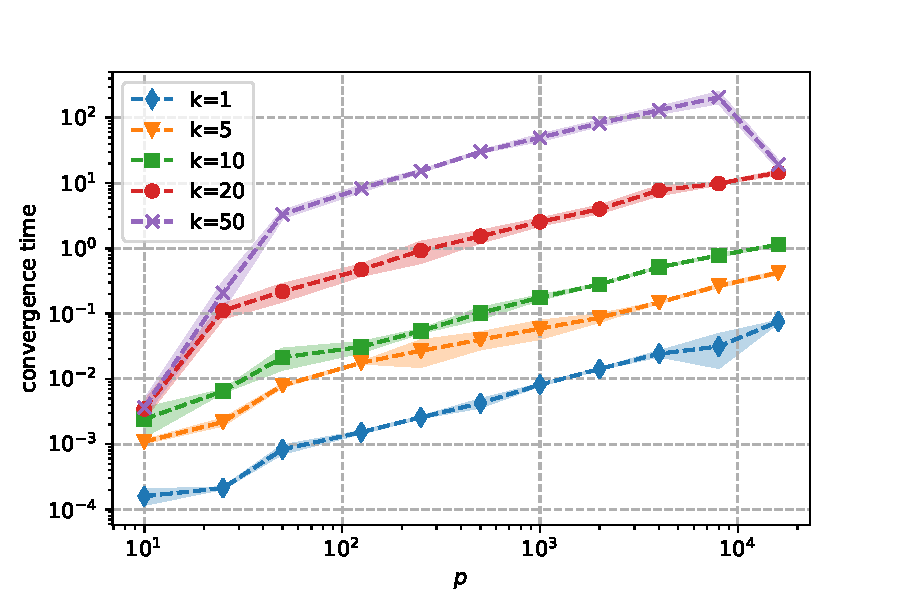
\includegraphics[width=0.8\linewidth, height=0.5\linewidth]{figures/low_rank_times.pdf}
    \caption{
        Convergence times of the low-rank coordinate ascent algorithm~\ref{alg:low_rank_coordinate_ascent}
        as a function of $p$ and $k$.
        It confirms the theoretical $\cO(n_{\text{iters}} \cdot p \cdot k^3)$ rate.
        In practice,
        the algorithm converges much faster to an appropriate solution when using a larger tolerance threshold.
        See Appendix~\ref{sec:coordinate_ascent_data} for details regarding the random data generation.
    }
    \label{fig:low_rank_times}
\end{figure}

This scheme is summarized in Algorithm~\ref{alg:low_rank_coordinate_ascent}.
It uses at most $\cO\left( p \cdot k \right)$ memory
and the time complexity is $\cO\left( n_\text{iters} \cdot p \cdot k^2 \right)$, as stated above.
We make a Cython implementation which is available in the released Python package.
Because of numerical instabilities, we completed experiments with a version inverting the matrix
$I_k + 2A_j$ at each iteration, leading to a higher time complexity of
$\cO\left( n_\text{iters} \cdot p \cdot k^3 \right)$.
Figure~\ref{fig:low_rank_times} shows the convergence times obtained in these experiments,
as a function of $p$ and $k$.
It demonstrates that the scalability is much better than with SCS,
thanks to the low-rank approximation and the fact that coordinate descent
is particularly well-suited to this optimization problem.
Even with $100\,000$ features, the convergence could be obtained in a few minutes.
We hope to prevent numerical instabilities in future versions and attain the
$\cO\left( n_\text{iters} \cdot p \cdot k^2 \right)$ time complexity.

\subsection{Efficient low-rank sampling}\label{subsec:low_rank_sampling}

In this section, we detail briefly how to sample knockoffs $\tcX$ once
a feasible solution $\bs$ is computed,
and in the special case where $\cove = D + U\Lambda U^\top$.
As shown in Section~\ref{subsec:gaussian_knockoffs},
$\tcX$ is sampled from the following conditional distribution
\begin{equation}\label{eq:conditional_gaussian_knockoffs3}
    \tcX \mid \cX \sim \cN\left( \bupsilon, \Upsilon \right)
    ,\qquad\text{where}\quad
    \begin{cases*}
        \bupsilon = \cX - \cX\Sigma^{-1}\diag\{ \bs \}\\
        \Upsilon = \diag\{ \bs \}\left( 2I_{p \times p} - \Sigma^{-1}\diag\{ \bs \} \right)
    \end{cases*}
\end{equation}
A classical approach to sample
$\zz \sim \cN\left( \bupsilon,\, \Upsilon \right)$
from a multivariate normal distribution is to sample first a vector
$\tilde{\zz} \in \R^p$ from $\cN\left( 0,\, 1 \right)$,
and then pose $\zz = \bupsilon + L\tilde{\zz}$,
where $L$ is a lower Cholesky factorization of $\Upsilon$.
This uses the fact that if $\xx \sim \cN\big( \mu,\, \Sigma \big)$,
then
\begin{equation}\label{eq:affine_transformation}
    A\xx + \bb \sim \cN\big( A\bmu + \bb,\, A\Sigma A^\top \big)
\end{equation}
Note that this scheme works even if $L$ is not lower-triangular,
but simply satisfies $LL^\top = \Upsilon$.

\bigbreak
As $\Upsilon$ is a $p \times p$ matrix we may not want to store it in memory,
nor compute a Cholesky factorization (which takes $\cO\left( p^3 \right)$ steps).
We show here how to factorize $\Upsilon$ in a cheap way,
requiring only $\cO\left( k \cdot p \right)$ memory and $\cO\left( k\cdot p^2 \right)$ operations.
We note $S = \diag\bs$, so that$\Upsilon = 2S - S\cove^{-1}S$.
Using the low-rank structure $\cove = D + U\Lambda U^\top$,
the Woodbury formula (see Appendix~\ref{sec:sherman}) gives
\begin{align*}
    \cove^{-1} &= (D + UU^\top)^{-1}\\
    &= D^{-1} - D^{-1}U(I_k + U^\top D^{-1}U)^{-1}U^\top D^{-1}
\end{align*}
Note $L \in \R^{k \times k}$ the lower Cholesky factorization of
$(I_k + U^\top D^{-1}U)^{-1}$ (which can be computed efficiently if $k$ is small),
$V = SD^{-1}UL \in \R^{p \times k}$,
and $C = 2S - SD^{-1}S$.
Then the covariance reduces to
\begin{equation*}
    \Upsilon = C + VV^\top
\end{equation*}
where $C$ is diagonal and $VV^\top$ has rank at most $k$.
$C$ is not necessarily psd, which will force us to sample from a complex normal distribution.
Let $H$ be a complex square-root of $C$ (thus, potentially with imaginary numbers on the diagonal),
and $P = H^{-1}V \in \R^{p \times k}$.
Then,
\begin{equation*}
    \Upsilon = H \left( I_{p \times p} + PP^\top \right) H^\top
\end{equation*}
$\left( I_{p \times p} + PP^\top \right)$ can be factorized in the following way.
Note
\begin{equation*}
    W = \left(I_{k \times k} + \sqrt{I_{k \times k} + P^\top P}\right)^{-1} \in \R^{k \times k}
\end{equation*}
where the square-root is a $k \times k$ matrix root (which can again be computed efficiently if $k$ is small).
Then
\begin{equation*}
    I_{p \times p} + PP^\top = BB^\top
    ,\qquad
    \text{where}
    \quad
    B = I_{p \times p} + PWP^\top
\end{equation*}
Finally, we note $M = HB$ and we have that $\Upsilon = MM^\top$.
$B$ is $p \times p$ but we never have to fully evaluate it;
instead only $W$ and $P$ can be stored and matrix multiplications are then at most $p \times k$.

$M$ is a complex matrix so we cannot directly use the property~\ref{eq:affine_transformation}.
But if $\cX \sim \cN(\0,\, I)$ and $\cY = i\cX$,
then $\operatorname{Im}\left( M\cY \right) \sim \cN(\0,\, MM^\top = \Upsilon)$.
Using this scheme, we can draw dozens of thousands knockoff samples in a few seconds without explicitely
building $\cove$ nor $\Upsilon$.
